\chapter{Theoretical Overview}
This chapter will explain terms and technologies associated with personalization and recommendation, mobile user interfaces and digital news applications, to form a basis of what is often used when creating a mobile news recommendation application.


\section{Mobile User Interface}
After the rise of the smart phone, mobile content consumption has seen an incredible growth and is still growing\cite{emarketer2012moretime}, making the mobile user interface more and more common to people everywhere. The focus here will be on the smart phone, and the iPhone in particular, but applies to a lot of other smart phones manufactured as well.

Mobile devices brings with it a lot of opportunities, but has its limitations as well, compared to a desktop computer, for instance. Mobile screens are smaller than PC screens and are often touch-based, making the design approach for a mobile user interface a lot different.

A PC screen can normally hold more information in one view than a mobile device, so to display the same amount of information on a mobile screen, several views needs to be used and some form of navigation logic between them needs to be established. Also on systems where a mouse is used, which accounts for most computers, the possibility of bringing up information when the mouse hovers over an element is widely used, but on mobile user interfaces with touch screens, the hover possibility is not an option, ergo another way of showing the same information has to be created. 

On the other hand a touch device has a lot of possibilities that are not available or not as intuitive on a standard desktop computer. With a touch device, a user interacts directly with the element on a screen, compared to using a mouse. Gestures like dragging, pinching, swiping etc. can make a mobile user interface intuitive and easy to use, and more similar to gestures people do with actual objects. For instance, a swipe to the side to flip a page, similar to flipping a page in a real newspaper, is a more authentic experience to the real life than moving the mouse cursor to a page, clicking the mouse button and holding it down, and then drag it to flip the page.

Also a lot of mobile touch devices can register a lot of different event triggers, like touches, gestures, and movements, to mention a few. It is possible to differentiate between a touch with two fingers versus a touch with four fingers, a swipe with one finger versus a swipe with three fingers, and these gestures can also be combined. For instance, a user can touch and hold a box on the screen with two fingers for one second to trigger an edit mode, and further move this box around by starting to swipe two fingers while still holding on to the box, to position it wherever the user prefers, and then place the box by removing the fingers from the screen. Another possibility is to use a gyroscope, to have movement trigger some event in the mobile user interface. If a mobile phone is placed on a table facing up, and the phone starts ringing, turning the phone face down can trigger the silent function, for instance.


\section{Personalization}

According to Cylogy, personalization is "the process of deciding - given a large set of possible choices - what has the highest value to an individual"\cite{personalization_overview}

\cite{thurman2012future} defines it as "A form of user-to-system interactivity that uses a set of technological features to adapt the content, delivery, and arrangement of a communication to individual users’ explicitly registered and/or implicitly determined preferences."

So in other words: "give the users what they want, without them asking for it."

\section{Recommender System}
\label{theoretical_overview_recommender_system}
A recommender system is a system that filters or narrows down a large data set to a smaller data set to fit a user's preference, by using one or more predefined methods.

Recommender systems are becoming widely used and is a necessary approach to deal with the ever growing information overload situation that are occurring nowadays. These systems can be found in many different domains, like online shopping, reading news, listening to music or streaming other types of visual media, like movies or series.

\subsection{Filtering}
When building a recommender system there are three main approaches to follow, namely content-based filtering, collaborative filtering or a hybrid of these two. 

\subsubsection{Content-based Filtering}
Content-based filtering is a filtering technique where the items proposed are chosen based on similar items to what the system thinks the user is interested in. The items have some sort of classifying meta data, that makes them comparable to other items, and the item with the best match to the user's profile will be the item proposed. The user profile can be built by extracting and classifying events from the user's click log, for instance, or by explicit data the user supplies in terms of categories of interest etc.

Content-based filtering is dependent on knowledge about the items to be able to classify and cluster them, and sophisticated methods based on machine learning and NLP are often used to fulfill this purpose. 


\subsubsection{Collaborative Filtering}
Collaborative filtering is a filtering technique that proposes items based on which items other similar users have been accessing. Often large amount of user data from other users' activities or preferences are gathered and analyzed and the users are put into segments based on their behavior. If a user from one segment accesses an item, this item can be proposed as a recommended item for another user within this segment.

An advantage of this approach as opposed to content-based filtering, is that collaborative filtering does not need to have an understanding of the item itself to be able to recommend it to a user. On the other hand, collaborative filtering often suffers from cold start\cite{lam2008addressing}-, scalability- and data sparsity\cite{huang2004applying} problems.

\subsubsection{Hybrid Filtering}
Hybrid filtering is an approach where content-based filtering and collaborative filtering are combined in some way, and it has shown that this approach is more effective in some cases, as presented in section \ref{related_work_personlized_news}.

One way of conducting the hybrid approach is to implement collaborative filtering and content-based filtering separately, and then combining them. Another way is to use some capabilities from one approach and add it to the other approach. One can also merge them together, and apply them as a single model.

\section{News Application}
A news application is an application where a user can access news digitally via the Internet from one or more news publishing sources. This application can be provided by the content publisher itself, or it can be provided by a third party redistributing the content.

News applications are becoming widely used, and the consumption of news are rapidly shifting towards accessing news online and via mobile devices (see figure \ref{pew_news_consumption_survey}).

\begin{figure}[!htbp]
\centering
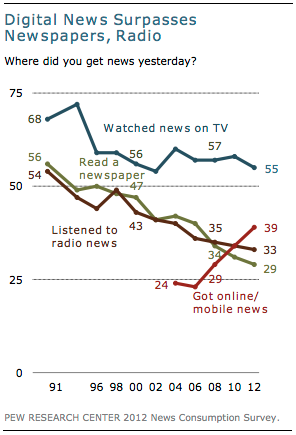
\includegraphics[width=70mm]{GFX/tech/pewNewsConsumptionSurvey.png}
\caption{The shifting of how people access news from 1991 to 2012 shown in percent of people asked.}
\label{pew_news_consumption_survey}
\end{figure}

\subsection{News Recommendation}
News recommendation is when a news application is combined with a recommender system, explained in section \ref{theoretical_overview_recommender_system}, to provide an online news reading user with a news service that are filtered or personalized to the user's preferences and likings.

A challenge with news recommendation, compared to for instance movie or music recommendation, is the freshness of the news. News have a short lifespan, and are best served fresh, making approaches like collaborative filtering a difficult task considering the cold start problem and data sparsity problem.

\subsection{Perspectives}
\label{theoretical_bg_perspectives}
There are a lot of different ways that news can be presented, considering how much information from a news article that are shown, how it is shown graphically, what the information shown means in different contexts etc. Following are description of the perspectives that are most used in different news applications and the applications referred to in this section will be further examined and presented in section \ref{commercial_news_applications}.

\subsubsection{Full Article}
A full article perspective, as the name implies, is perspective that normally holds all the information available for that particular news story. The most important information in this perspective is the full article text, as this is the information that most often is lacking in the other perspectives. Figure \ref{full_article_prismatic} shows an example of a full article perspective.

\begin{figure}[!htbp]
\centering
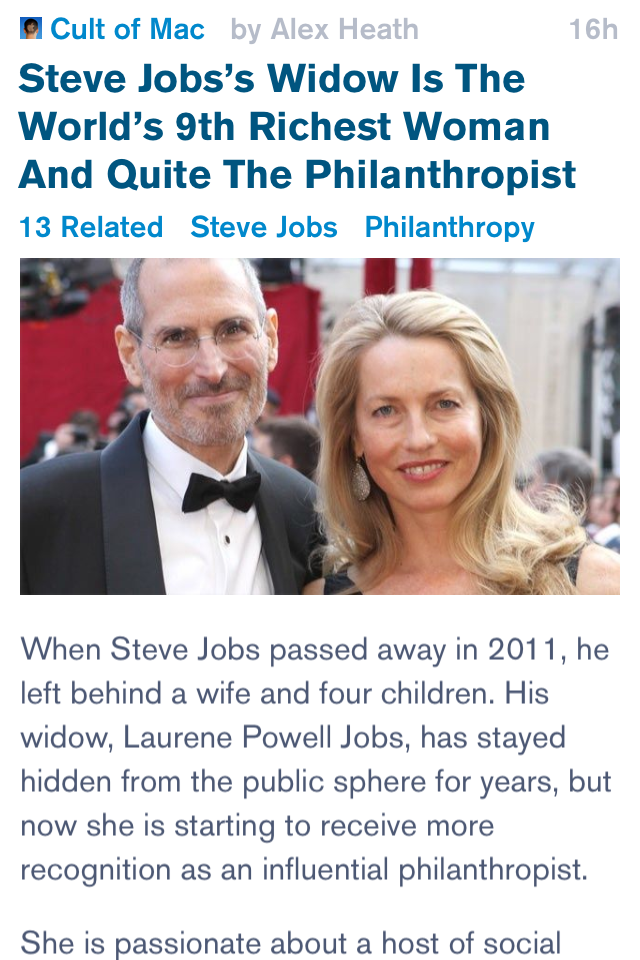
\includegraphics[width=50mm]{GFX/perspectives/fullArticleViewPrismatic.png}
\caption{A screenshot from Prismatic showing an example of a full article perspective.}
\label{full_article_prismatic}
\end{figure}

\subsubsection{RSS}
An RSS perspective is a perspective showing just some of the information from an article to give the user a quick overview of what the news article concerns. The name stems from the RSS feed technology which has a certain set of information like title, lead-text, when the article was published, and sometimes an image. The RSS view may have other information as well, but the ones mentioned are the most common. Figure \ref{rss_feedly} shows an example of how an RSS perspective may be presented.

\begin{figure}[!htbp]
\centering
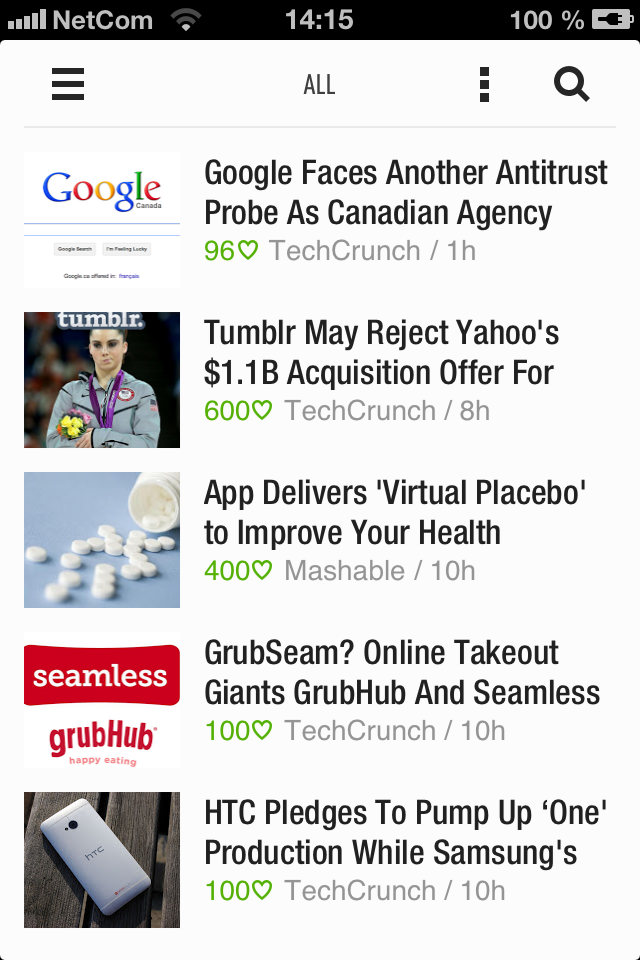
\includegraphics[width=50mm]{GFX/perspectives/rssViewFeedly.png}
\caption{A screenshot from Feedly showing an example of an RSS perspective.}
\label{rss_feedly}
\end{figure}

\subsubsection{Entity}
An entity perspective is a perspective showing a set of keywords extracted from a news article by the use of a keyword extracting algorithm or other NLP technologies. Figure \ref{entity_news_cloud} shows an example of how an entity perspective can be displayed to the user. In this application if a keyword is selected, all the other keywords that are connected to this keyword is highlighted. The articles these keywords are extracted from are shown in a view on the right-hand side as links that will take the user to the corresponding article if clicked.

\begin{figure}[!htbp]
\centering
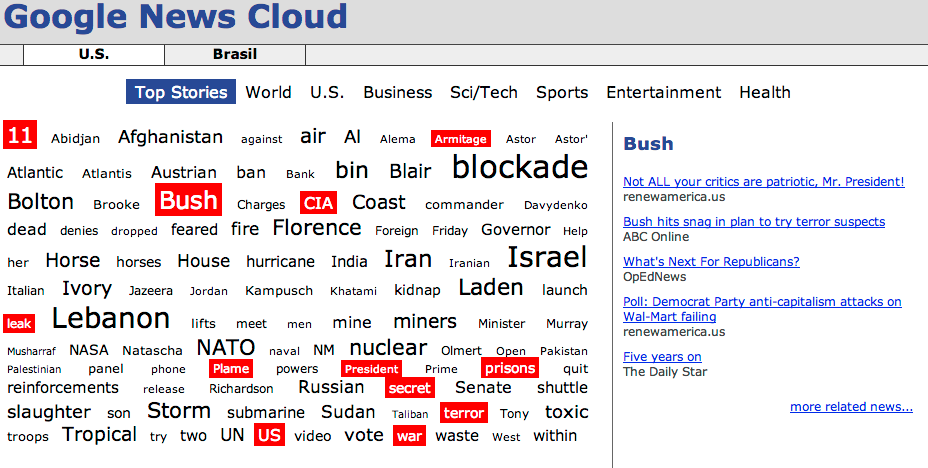
\includegraphics[width=140mm]{GFX/perspectives/entityViewNewsCloud.png}
\caption{A screenshot from NewsCloud showing an example of an entity perspective.}
\label{entity_news_cloud}
\end{figure}

\subsubsection{Event}
An event perspective is a perspective that displays certain events that occurred by analyzing news articles and extracting those events by using NLP or other text-analyzing techniques. Figure \ref{event_wavii} shows three events extracted from different news articles. The first shows that two celebrities broke up, the second shows that a theatrical trailer was released by a movie publisher and the third shows that a software company released a new application for the iOS platform.

\begin{figure}[!htbp]
\centering
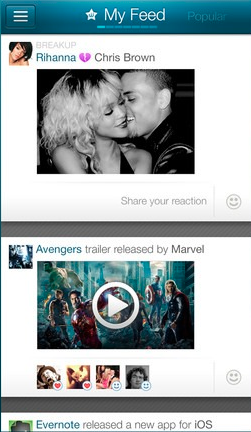
\includegraphics[width=50mm]{GFX/perspectives/eventViewWavii.png}
\caption{A screenshot from Wavii showing an example of an event perspective.}
\label{event_wavii}
\end{figure}

\subsubsection{Web}
The web perspective is quite similar to the full article perspective and usually includes the same amount of information. The main difference is that the web perspective is the news article shown at the publisher's website through an application by the use of a web browser inside a third party application. This is a widely used perspective as a third party application cannot normally show a full news article from another publisher without an agreement with the publisher itself. Showing a full article without a contract with the publisher is most likely a copyright infringement. Figure \ref{web_flipboard} shows an example of how a web perspective may be presented.

\begin{figure}[!htbp]
\centering
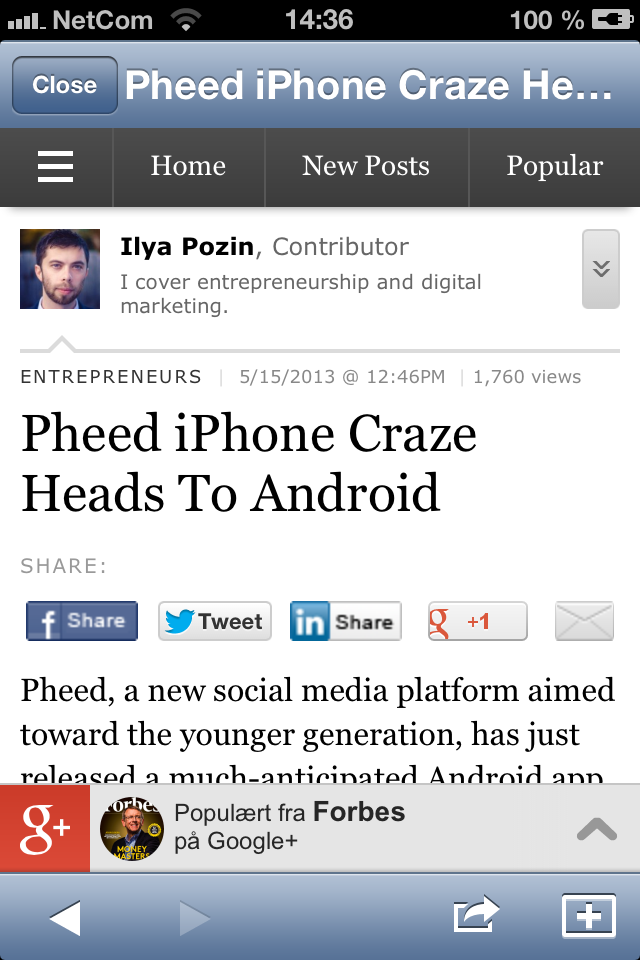
\includegraphics[width=50mm]{GFX/perspectives/webViewFlipboard.png}
\caption{A screenshot from Flipboard showing an example of a web perspective.}
\label{web_flipboard}
\end{figure}

\subsubsection{Summary}
The summary perspective is a perspective that shows a summary text of the full article text, where this text is created by the use of NLP technologies, like the Summly application, or hand crafted by real editors, like the Circa application. Figure \ref{summary_summly} shows a screenshot of the Summly application presenting a summary perspective.

\begin{figure}[!htbp]
\centering
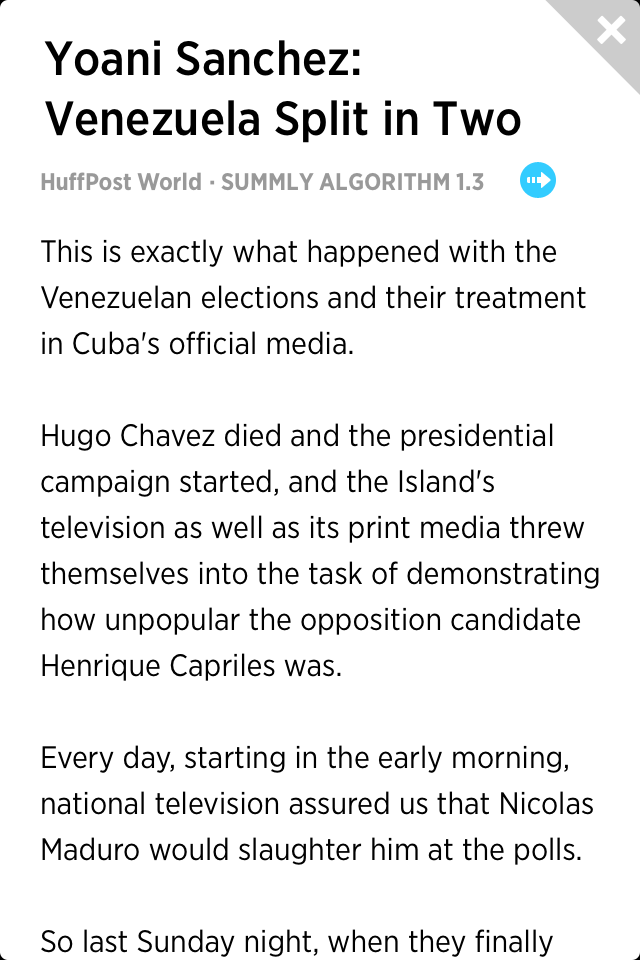
\includegraphics[width=50mm]{GFX/perspectives/summaryViewSummly.png}
\caption{A screenshot from Summly showing an example of a summary perspective.}
\label{summary_summly}
\end{figure}

\subsubsection{Map}
The map perspective is a perspective that shows where in the world a news story concerns by the use of a map view. Figure \ref{map_circa} shows a news story residing in Lisbon, Portugal in the Circa application.

\begin{figure}[!htbp]
\centering
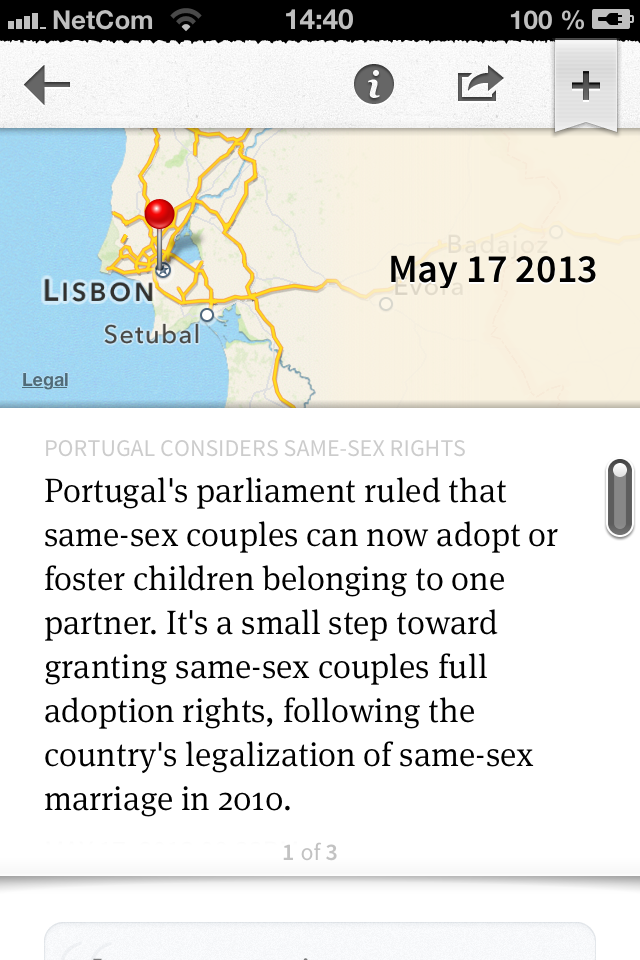
\includegraphics[width=50mm]{GFX/perspectives/mapViewCirca.png}
\caption{A screenshot from Circa showing an example of a map perspective.}
\label{map_circa}
\end{figure}

